\chapter{Proposed Solution}\label{ch:proposed-solution}

This chapter will discuss the methods this work considers to recognise the outer \(k\)-planar graphs. Besides recognition, these methods provide the outer \(k\)-planar drawings of the given graphs if possible. We represent the drawing as a sequence of vertices in the circular order in which they appear on the boundary of the outer face.

For operations with graphs, we use C++ Boost Graph Library~\cite{boost}. As a graph class, we use \textsf{adjacency\_list} as for all methods described below, we require both \textsf{VertexList} and \textsf{EdgeList} concepts to be able to iterate over both vertices and edges. We prefer this class to an \textsf{adjacency\_matrix} as, according to the documentation\footnote{\url{https://www.boost.org/doc/libs/1_88_0/libs/graph/doc/adjacency_matrix.html}}, it trades memory consumption and speed of graph traversal for the speed of edge insertion and deletion, and neither of these operations is used for algorithms described below.

\todo[inline]{Explicily specify the goals of the work: implement three algorithms, provide an interface.}


\section{Bicomponent decomposition}

\begin{figure}
    \centering
    \subcaptionbox{An original graph with highlighted biconnected components and cut vertices \label{fig:bidec:original_graph}} {
        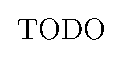
\includegraphics[width=0.4\textwidth]{TODO}
    }
    \hfill
    \subcaptionbox{Block-cut tree of a graph \label{fig:bidec:bctree}} {
        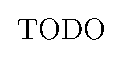
\includegraphics[width=0.4\textwidth]{TODO}
    }
    \hfill
    \subcaptionbox{Outer \(k\)-planar drawing of each component \label{fig:bidec:componnents_drawings}}{
        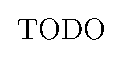
\includegraphics[width=0.4\textwidth]{TODO}
    }
    \hfill
    \subcaptionbox{
        Outer \(k\)-planar drawing of the original graph \label{fig:bidec:graph_drawing}} {
        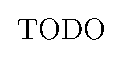
\includegraphics[width=0.4\textwidth]{TODO}
    }
    \caption{An example of bicomponent decomposition}
\end{figure}

For complex problems, a decomposition into smaller subproblems often leads to a significant increase in performance. In our context of recognising outer \(k\)-planar graphs, an effective strategy to do so is to partition the graph into subgraphs in such a manner that allows us to process each part independently by the recognition algorithm. One of the plausible ways to accomplish this is to split the graph into biconnected components as shown in figure~\ref{fig:bidec:original_graph} using block-cut decomposition. It is worth noting that each edge of the graph belongs to a single biconnected component, referred to as a block. However, any two bicomponents may share a vertex, referred to as a cut vertex. Considering blocks and cut vertices as graph nodes, we can construct a so-called block-cut tree, wherein a block node is connected to a cut node if and only if the corresponding biconnected component contains a corresponding cut vertex, see figure~\ref{fig:bidec:bctree}.

Due to the nature of bi-connectedness, after getting outer \(k\)-planar drawings of biconnected components separately, we can combine them easily into an outer \(k\)-planar drawing of the whole graph, hence, \todo{How to show this more formally?} the increase in performance. To be more specific, if some component does not admit an outer \(k\)-planar drawing, neither does the whole graph. Otherwise, if all components admit such a drawing, they can be merged by combining duplicates of each cut vertex see figures~\ref{fig:bidec:componnents_drawings} and~\ref{fig:bidec:graph_drawing}. This merging process does not introduce any additional edge crossings since both components are located on the outer face of each other. Moreover, as no new faces are created during this process (due to the acyclic structure of the block-cut tree), every vertex remains on the outer face of the graph during this process. Consequently, the resulting drawing of an original graph is outer \(k\)-planar, and it exists if and only if each biconnected component of the graph admits such a drawing.

In\todo{Do we really need this here? I have mentioned Boost in the introduction to the chapter} this work, we implemented this decomposition using the method \textsf{bi\-connec\-ted\_compo\-nents}\footnote{\url{https://www.boost.org/doc/libs/1_87_0/libs/graph/doc/biconnected_components.html}} from the Boost Graph Library~\cite{boost}. This function assigns an index of the bicomponent to each edge to which it belongs. Additionally, it provides a list of cut vertices. Afterwards, we copy each block as an independent graph and create mappings to translate new \emph{local} vertices back to their original identifiers. Finally, we construct a supergraph representing the structure of a block-cut tree wherein each node references a copied block alongside corresponding mapping or a cut vertex.

To construct a drawing of the whole graph, after performing the decomposition, we perform a depth-first search on the block-cut tree, recording the predecessor for each node upon discovery. Additionally, each time a block vertex is discovered, we use one of the methods described in other sections of this chapter to check whether the component admits an outer \(k\)-planar drawing and obtain it if so. Afterwards, we merge the new drawing with the already existing one by combining the common cut vertex if such exists. To be more specific, if the considered block is the first encountered one, its drawing is directly copied into a sequence that will form the final drawing. Otherwise, the block necessarily has a predecessor. Due to the structure of a tree, it is a cut node corresponding to a vertex that is shared with some other block. Due to how we traverse the tree, that other block has already been considered and thus added to a final drawing. As a result, the corresponding cut vertex is present in both global and local drawings. Since each drawing is represented as a cyclic sequence of vertices, we can rotate the local one so that the corresponding cut vertex appears as the first one in a sequence. Finally, we insert the local drawing starting from the second element into the global one immediately after the corresponding cut vertex.


\section{ILP-based algorithm}\label{sec:ILP-def}

As the problem of recognising the outer \(k\)-planar graphs is NP-hard, it can be reduced to another NP-hard problem. Some of them have already been studied for decades. During this period, extremely optimised algorithms for their solving have emerged. One of them is an Integer Linear Programming problem~(ILP). This problem asks to find a realisation of a variable vector \(\mathbf{x}\) that optimises the objective represented as a linear combination of variables \(\mathbf{c}^T\mathbf{x}\) subject to specific constraints \(\mathbf{Ax}\leqslant\mathbf{b}\). Additionally, some variables in the ILP problem are restricted to integer values. Since researchers have extensively studied the problem and developed efficient solvers, we decided to use their results to build an algorithm for recognising outer \(k\)-planar graphs. In this section, we discuss the details of the reduction we considered for our problem to the ILP\@. As an implementation of ILP solver, we used Gurobi Optimizer~\cite{gurobi} under the free academic licence\todo{Explain why we have chosen Gurobi}.

To reduce a recognition problem to an ILP, we have to represent its structure using variables and constraints. We start with a graph drawing, which is represented, as described above, as a sequence of vertices. For the ILP, we can encode it using the so-called ``ordering variables'', which indicate a relative order of two vertices. Specifically, for every pair of vertices \(u\) and \(v\), we create a binary variable \(a_{u, v}\) introducing a constraint~\eqref{eq:ilp:con:order-var}. We interpret the value \(1\) as an indication of vertex \(u\) being located before vertex \(v\) and the value \(0\) as an indication of either \(v\) being located before \(u\) or \(u\) and \(v\) being the same vertex.

To ensure that these variables encode a valid sequence, we also have to enforce the transitivity. That is, for every ordered pair of distinct vertices \(u\) and \(v\), and every other vertex \(w\), if \(a_{u, w} \equiv 1\) and \(a_{w, v} \equiv 1\), meaning \(u\) is located before \(w\) and \(w\) is located before \(v\), then \(u\) must be located before \(v\), so the following should hold \(a_{u, v} \equiv 1\). Including also the implication for the reversed order, we get:
\begin{align}
    a_{u, w} \equiv 1 \land a_{w, v} \equiv 1 \longrightarrow a_{u, v} \equiv 1 \label{eq:ilp:transitivity:uv:1}\\
    a_{u, w} \equiv 0 \land a_{w, v} \equiv 0 \longrightarrow a_{u, v} \equiv 0 \label{eq:ilp:transitivity:uv:0}
\end{align}
If we instead consider a pair \(v, u\) and the same vertex \(w\),  the constraints would look like follows:
\begin{align}
    a_{v, w} \equiv 1 \land a_{w, u} \equiv 1 \longrightarrow a_{v, u} \equiv 1 \label{eq:ilp:transitivity:vu:1} \\
    a_{v, w} \equiv 0 \land a_{w, u} \equiv 0 \longrightarrow a_{v, u} \equiv 0 \label{eq:ilp:transitivity:vu:0}
\end{align}
Note that for any distinct vertices \(x\) and \(y\) the equality \(a_{x, y} = 1 - a_{y, x}\) always holds, thus equations~\eqref{eq:ilp:transitivity:uv:1} and~\eqref{eq:ilp:transitivity:vu:0} alike equations~\eqref{eq:ilp:transitivity:uv:0} and~\eqref{eq:ilp:transitivity:vu:1} are equivalent. Consequently, it is enough to ensure only the first constraint as long as we do it for every ordered pair of vertices. Considering that the variables are binary, to limit \(a_{u, v}\) to \(1\) it is enough to impose a constraint \(a_{u, v} \geqslant \epsilon\) for any \(\epsilon \in (0;1]\). In a constraint for ILP, this \(\epsilon\) must be represented as a linear function of \(a_{u, w}\) and \(a_{w, v}\). The values of this function must lie in the half-interval \((0;1]\) if and only if both binary variables are \(1\). Using an expression \(a_{u, v} + a_{v, w} - 1\) for this leads to a constraint~\eqref{eq:ilp:con:transitivity} in the ILP formulation.

\begin{figure*}
    \centering
    \subfloat[][]{
\includegraphics[width=.3\textwidth]{edge_cross/uvst}} \hfill
    \subfloat[][]{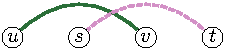
\includegraphics[width=.3\textwidth]{edge_cross/usvt}\label{fig:edge_crossings:example-cross}} \hfill
    \subfloat[][]{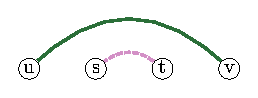
\includegraphics[width=.3\textwidth]{edge_cross/ustv}} \hfill
    \subfloat[][]{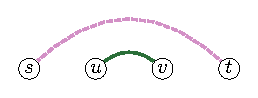
\includegraphics[width=.3\textwidth]{edge_cross/suvt}} \hfill
    \subfloat[][]{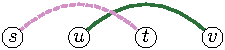
\includegraphics[width=.3\textwidth]{edge_cross/sutv}} \hfill
    \subfloat[][]{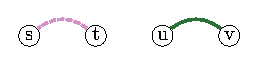
\includegraphics[width=.3\textwidth]{edge_cross/stuv}} \hfill

    \subfloat[][]{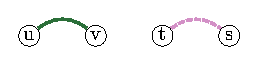
\includegraphics[width=.3\textwidth]{edge_cross/uvts}} \hfill
    \subfloat[][]{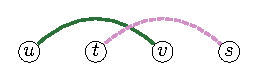
\includegraphics[width=.3\textwidth]{edge_cross/utvs}} \hfill
    \subfloat[][]{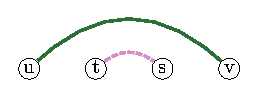
\includegraphics[width=.3\textwidth]{edge_cross/utsv}} \hfill
    \subfloat[][]{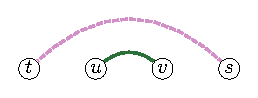
\includegraphics[width=.3\textwidth]{edge_cross/tuvs}} \hfill
    \subfloat[][]{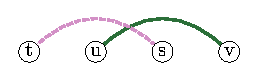
\includegraphics[width=.3\textwidth]{edge_cross/tusv}} \hfill
    \subfloat[][]{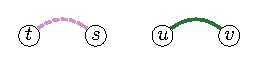
\includegraphics[width=.3\textwidth]{edge_cross/tsuv}} \hfill

    \subfloat[][]{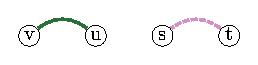
\includegraphics[width=.3\textwidth]{edge_cross/vust}} \hfill
    \subfloat[][]{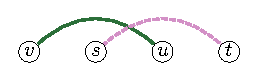
\includegraphics[width=.3\textwidth]{edge_cross/vsut}} \hfill
    \subfloat[][]{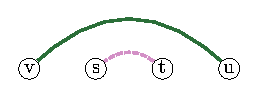
\includegraphics[width=.3\textwidth]{edge_cross/vstu}} \hfill
    \subfloat[][]{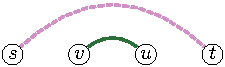
\includegraphics[width=.3\textwidth]{edge_cross/svut}} \hfill
    \subfloat[][]{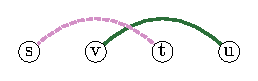
\includegraphics[width=.3\textwidth]{edge_cross/svtu}} \hfill
    \subfloat[][]{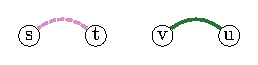
\includegraphics[width=.3\textwidth]{edge_cross/stvu}} \hfill

    \subfloat[][]{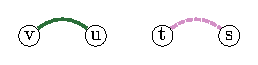
\includegraphics[width=.3\textwidth]{edge_cross/vuts}} \hfill
    \subfloat[][]{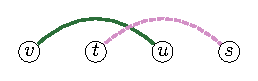
\includegraphics[width=.3\textwidth]{edge_cross/vtus}} \hfill
    \subfloat[][]{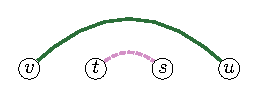
\includegraphics[width=.3\textwidth]{edge_cross/vtsu}} \hfill
    \subfloat[][]{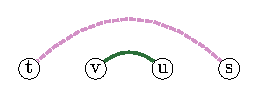
\includegraphics[width=.3\textwidth]{edge_cross/tvus}} \hfill
    \subfloat[][]{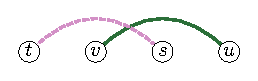
\includegraphics[width=.3\textwidth]{edge_cross/tvsu}} \hfill
    \subfloat[][]{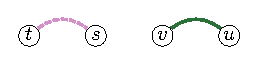
\includegraphics[width=.3\textwidth]{edge_cross/tsvu}}
    \caption{All \(24\) possible arrangements of two edges' endpoints, only \(8\) of which result in intersection. \emph{I do not think it is really necessary. It is TOO big}}
    \label{fig:edge_crossings}
\end{figure*}

The next step of the algorithm is to encode the intersections. To represent them, for every unordered pair of edges, \(uv\) and \(st\), we introduce a binary variable \(c_{uv, st}\), hence the constraint~\eqref{eq:ilp:con:cross-var}. The endpoints of the edges can be arranged in \(24\) different ways, among which only eight result in an intersection, as demonstrated in figure~\ref{fig:edge_crossings}. To encode this, we must ensure that the value of the variable \(c_{uv, st}\) equals \(1\) if the corresponding ``ordering variables'' indicate one of these eight arrangements\footnote{As the objective of the program is to minimise the number of crossings, we do not constraint \(c_{uv, st}\) to \(0\) when \(uv\) and \(st\) do not cross leaving it to the optimiser. Doing so, we simplify the problem by reducing the number of constraints for every pair of edges from \(24\) to \(8\).}. For example, considering the arrangement in figure~\ref{fig:edge_crossings:example-cross}, we have to limit the value of \(c_{uv, st}\) to \(1\) if the endpoints are arranged in the order \(usvt\). This order of vertices is implied by the model if and only if each equivalence out of \(a_{u,s} \equiv 1\), \(a_{s,v} \equiv 1\) and \(a_{v,t} \equiv 1\) holds. Thus, we can represent this limitation as follows:
\begin{align*}
    a_{u,s} \equiv 1 \land a_{s,v} \equiv 1 \land a_{v,t} \equiv 1 \longrightarrow c_{uv, st} \equiv 1
\end{align*}
To transform it into a constraint for an ILP formulation, we can use the same logic as for encoding the equation~\eqref{eq:ilp:transitivity:uv:1}, getting as a result the constraint~\eqref{eq:ilp:con:cross-example}. The constraints~\eqref{eq:ilp:con:cross-begin} to~\eqref{eq:ilp:con:cross-end} are constructed analogously for the other seven intersecting arrangements.

Lastly, the algorithm has to encode each edge's crossing number and minimise the maximal value out of them. The crossing number of each edge can be easily represented as a sum of the corresponding ``crossing variables'':
\begin{align}
    \label{eq:ilp:crossing-number}
    cr_{e_1} \leqslant \sum_{e_2 \in E(G)} c_{e1, e2}
\end{align}
However, as the maximum is not a linear function, constructing the objective function out of the per-edge crossing numbers is not as simple. To get around this limitation, we have to introduce a new continuous variable \(k\), which represents the crossing number of the whole graph \(G\). To ensure that, we have to bound \(k\) from below by the crossing number of each edge: \(k \geqslant cr_{e_1} \forall e_1 \in E(G)\). Combining this with inequality~\eqref{eq:ilp:crossing-number}, we get the constraint~\eqref{eq:ilp:con:crossing-number}. As a result, minimising for \(k\) would give the desired result.

Combining everything together, we get the following formulation of the ILP problem:
\begin{align}
    \textbf{minimize}\quad&k  \label{eq:ilp:objective}\\
    \textbf{subject to}\quad
    &&a_{u, v} &\geqslant a_{u, w} + a_{w, v} - 1,&&\forall u, v, w \in V(G)  \label{eq:ilp:con:transitivity}\\
    &&c_{uv, st} &\geqslant a_{u,s} + a_{s,v} + a_{v,t} - 2,&&\forall uv, st \in E(G)  \label{eq:ilp:con:cross-example}\\
    &&c_{uv, st} &\geqslant a_{u,t} + a_{t,v} + a_{v,s} - 2,&&\forall uv, st \in E(G) \label{eq:ilp:con:cross-begin}\\
    &&c_{uv, st} &\geqslant a_{v,s} + a_{s,u} + a_{u,t} - 2,&&\forall uv, st \in E(G)\\
    &&c_{uv, st} &\geqslant a_{v,t} + a_{t,u} + a_{u,s} - 2,&&\forall uv, st \in E(G)\\
    &&c_{uv, st} &\geqslant a_{s,u} + a_{u,t} + a_{t,v} - 2,&&\forall uv, st \in E(G)\\
    &&c_{uv, st} &\geqslant a_{t,u} + a_{u,s} + a_{s,v} - 2,&&\forall uv, st \in E(G)\\
    &&c_{uv, st} &\geqslant a_{s,v} + a_{v,t} + a_{t,u} - 2,&&\forall uv, st \in E(G)\\
    &&c_{uv, st} &\geqslant a_{t,v} + a_{v,s} + a_{s,u} - 2,&&\forall uv, st \in E(G)  \label{eq:ilp:con:cross-end}\\
    &&k &\geqslant \sum_{st \in E(G)} c_{uv, st},&&\forall uv \in E(G)  \label{eq:ilp:con:crossing-number}\\
    &&c_{uv, st} &\in \{0, 1\},&&\forall uv, st \in E(G)  \label{eq:ilp:con:cross-var}\\
    &&a_{u, v} &\in \{0, 1\},&&\forall u, v \in V(G)  \label{eq:ilp:con:order-var}
\end{align}

After encoding the problem as an ILP problem, as we described above, we run the ILP solver. After optimisation, it returns assigned values for each variable used in the program. The variables of interest for us are ``ordering variables'' \(a_{u, v}\) and \(k\). The latter one indicates the minimal possible crossing number that is reported. The former one we use to reconstruct an outer \(k\)-planar drawing of the original graph. As the desired drawing is a sequence of vertices, we must order them. To do so, we can use the values of ``ordering variables'' to define the strict total order relation. We say that for two vertices \(u\) and \(v\) \(u < v\) if and only if \(a_{u, v}\) is assigned to \(1\). Due to the construction of these variables and transitivity constraint~\eqref{eq:ilp:con:transitivity}, this order satisfies all requirements of the strict total order. Thus, it can sort the vertices, resulting in an outer \(k\)-planar drawing.


\section{SAT-based algorithm}\label{sec:SAT-def}

Another example of a thoroughly studied NP-hard problem is a Boolean Satisfiability problem~(SAT). As an input, the problem gets a boolean formula in a conjunctive normal form~(CNF). For the output, it asks for such an assignment of logic values \textsc{True} and \textsc{False} to the variables used in the input, such that the expression evaluates to \textsc{True}. In this section, we discuss the details of the reduction of the recognition problem to the SAT one. To do so, we represent our problem as a boolean expression, which is satisfied if and only if the graph admits an outer \(k\)-planar drawing. As an implementation of SAT solver, we used kissat~\todo{I can not find DOI for this article, so bib emtry looks different}\cite{kissat, kissat-library}\todo{Explain why we have chosen kissat}.

To encode the drawing, we use the ``ordering variables'' \(a_{u, v}\) we used in the ILP-based algorithm described in the section~\ref{sec:ILP-def} interpreting the value \(1\) as \textsc{True} and \(0\) as \textsc{False}. To encode the transitivity constraint, we follow the same logic, ending up with the same implication~\eqref{eq:ilp:transitivity:uv:1}. In terms of boolean algebra, this can be encoded as follows:
\begin{align*}
    a_{u, v} \land a_{v, w} \rightarrow a_{u, w}
\end{align*}
To transform this into CNF, we expand the implication and apply De Morgan's law, getting the first set of clauses in the SAT representation:
\begin{align}
    a_{u, v} \land a_{v, w} \rightarrow a_{u, w}
    &\equiv \overline{(a_{u, v} \land a_{v, w})} \lor a_{u, w} \nonumber \\
    &\equiv \overline{a_{u, v}} \lor \overline{a_{v, w}} \lor a_{u, w} \label{sat:trans}
\end{align}

To encode the edges' intersections, we also reuse ``crossing variables'' \(c_{uv, st}\) from ILP reduction. Similarly, we ensure that the variable is set to \textsc{True} if the endpoints of the corresponding edges are arranged in one of eight crossing patterns (see figure~\ref{fig:edge_crossings}). This leads to eight sets of clauses, each of which contains ones representing one of these arrangements for all ``crossing variables''. For example, for the arrangement from figure~\ref{fig:edge_crossings:example-cross} the constraint for the variable \(c_{uv, st}\) can be encoded as follows:
\begin{align*}
    a_{u,s} \land a_{s,v} \land a_{v,t} \rightarrow c_{uv, st}
\end{align*}
To get a clause out of it, we expand the implication and apply De Morgan's law:
\begin{align}
    a_{u,s} \land a_{s,v} \land a_{v,t} \rightarrow c_{uv, st}
    & \equiv \overline{a_{u,s} \land a_{s,v} \land a_{v,t}} \lor c_{uv, st} \nonumber \\
    & \equiv \overline{a_{u,s}} \lor \overline{a_{s,v}} \lor \overline{a_{v,t}} \lor c_{uv, st} \label{sat:crossing-vars}
\end{align}

The last thing to encode is the limit of \(k\) intersections per edge. Unlike ILP reduction, we cannot add the corresponding variable. To impose this restriction, we ensure that no edges are crossed at least \(k+1\) times. For that, for each edge \(e_0\) and every set of \(k+1\) edges \(E = \{e_1, e_2, \dots, e_{k+1}\}\) we add a following clause to the boolean formula:
\begin{align}
    \overline{c_{e_0, e_1}} \lor \overline{c_{e_0, e_2}} \lor \cdots \lor \overline{c_{e_0, e_{k+1}}} \label{sat:cr-limit}
\end{align}
which evaluates to \textsc{True} if and only if at least one variable is set to \textsc{False}. By inserting this clause for every possible set \(E\), we ensure that no \(k+1\) edges cross the same edge. Thus, if the resulting boolean expression is satisfiable by some realisation of the variables, the values of ``ordering variables'' from this realisation would indicate an outer \(k\)-planar drawing.

Lastly we combine clauses~\eqref{sat:trans} for all triplets of vertices \(u\), \(v\) and \(w\), with clauses~\eqref{sat:crossing-vars} for all pairs of edges \(uv\) and \(st\), and with clauses~\eqref{sat:cr-limit} for all edges \(e_0\) and all sets \(E\) of \(k+1\) edges. We combine the clauses using logical and operator (\(\land\)), as every single clause must be satisfied to graph to be outer \(k\)-planar. Then, we run the SAT solver using the resulting boolean expression as an input. If the solver fails to find a satisfiable instance, the algorithm halts, indicating that the graph is not outer \(k\)-planar. Otherwise, the algorithm halts returning the desired graph drawing. To reconstruct an outer \(k\)-planar drawing, similar to reduction to an ILP problem, we sort the vertices using the values of the ``ordering variables'' assigned by the solver to specify the order.

Unfortunately, unlike reduction to an ILP, this one does not solve the optimisation problem of finding the minimal possible \(k\). The resulting algorithm solves the decision problem~--~whether the graph admits an outer \(k\)-planar drawing or not. To transform this into an optimisation, we incrementally check each integer, starting from \(0\), until the boolean expression becomes satisfiable.


\section{Optimisations for ILP and SAT algorithms}\label{sec:optimisations}

\todo[inline]{Not ready at all.}

In addition to the described reduction, we also considered a small optimisation for the objective function. In the implementation we discussed, we only ensure that each ``crossing variable'' equals \(1\) if two edges actually cross, so for any non-crossing edges, the variable might take on both \(0\) and \(1\). As the variables' influence on the objective is not direct, but through a constraint on the variable \(k\), it might be hard for an optimiser to estimate the influence of each variable accurately. To help it, we included an extra term in the objective function~\eqref{eq:ilp:objective}: \(\frac{\sum c_{e_1, e_2}}{|E|^2}\). By using \(|E|^2\) as a dominator in the fraction, we ensure that the value of the inserted term never exceeds \(1\) so that the optimiser would always prioritise decreasing \(k\) over this term.


\section{DP algorithm}

The last algorithm we considered was introduced by \citeauthor{okp}~\cite{okp}. Unlike previously discussed ones, this algorithm was explicitly designed to solve the recognition problem. This method uses the approach of dynamic programming, where the solution for a problem is built based on solutions of similar but smaller problems. Thus, the final drawing of the graph is built incrementally each time for a larger part of the original graph.

\begin{figure}
    \centering
    \captionsetup{subrefformat=parens}
    \subfloat[]{\label{fig:okp:config-graph}
    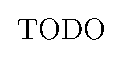
\includegraphics[width=0.4\textwidth]{TODO}
    }
    \hfill
    \subfloat[]{\label{fig:okp:triangle}
    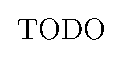
\includegraphics[width=0.4\textwidth]{TODO}
    }
    \caption{
        An example of \protect\subref{fig:okp:config-graph}~a graph \(G_{uv, R_{uv}}\) representing a configuration and \protect\subref{fig:okp:triangle}~a corresponding triangle.
        \emph{Something similar to\cite[Figure 4]{okp}}
    }
\end{figure}

The whole process can be divided into steps. Each one of them can be parameterised by three parameters. The first is a pair of vertices \(u\) and \(v\) that split a graph into two parts, denoted as a link. The next is a set \(R_{uv}\) of vertices lying to the right of the link. And lastly the set \(E_{uv} = \{e_1, e_2, \dots, e_l\}\) of \(l\) edges crossing the \(uv\) link from the right to the left side. To represent each step separately, we introduce a graph \(G_{uv, R_{uv}}\) (see figure~\ref{fig:okp:config-graph}) which consists of vertices \(\{u, v\} \cup R_{uv}\) alongside all connecting edges from an original graph \(G\) with inserted vertices \(t_1, t_2, \dots, t_l\) connected to corresponding vertices by edges \(e_1, e_2, \dots, e_l\). We call a configuration on each step \emph{drawable} if exists an outer \(k\)-planar drawing of a corresponding graph \(G_{uv, R_{uv}}\) which cyclic order contains \((u, t_{\tau(1)}, t_{\tau(2)}, \dots, t_{\tau(l)}, v)\) as a consecutive subsequence for some permutation \(\tau\). On each step, the algorithm finds all possible permutations for which the configuration is \emph{drawable} and stores them in the lookup table.

In the implementation of the algorithm, we first construct an index of all possible configurations. It allows us to simply iterate through it later without searching for the next configuration. Since, on each step, we try to draw a configuration using two smaller \emph{drawable} ones, we group them by the size of the right part, guaranteeing that all smaller \emph{drawable} configurations are already discovered at any point of the process. Unfortunately, it is unfeasible to consider all possible configurations due to the sheer number of them. For a graph with \(n\) vertices, there are \(\frac{n(n-1)}{2}\) links with \(2^{n-2}\) possible right sides each. As the link together with the right side uniquely determines the edges that cross the link, totally there are \(n(n-1)\cdot2^{n-3}\) possible configurations.

To significantly reduce the search space, the authors used the result of \citeauthor{triangulations}. They showed~\cite{triangulations} that there is a vertex \(w\) from the right side of any \emph{drawable} configuration that splits it into two smaller \emph{narrow} configurations for which \(|E_{uw}| \leqslant k\) and \(|E_{vw}| \leqslant k\). By reversing their argument, we get that \(G_{uv, R_{uv}}\) admits an outer \(k\)-planar drawing if and only if we can combine it from two \emph{narrow drawable} configurations. This allows us to limit the considered configurations only to \emph{narrow} once, reducing their number to~\(2^{O(k)}m^{k+O(1)}\)~\cite[Lemma 15]{okp} instances.

Despite this optimisation, there is still a massive number of configurations. To minimise the memory consumption and make it feasible, we represent the right sides as binary masks stored as 64-bit integers. This decision limits the current implementation to graphs with at most 64 vertices. However, considering the complexity of the algorithm, we believe the graphs of bigger sizes would require an unreasonable amount of resources anyway\footnote{Potentially it is possible to develop a specified bitmask object which could handle any number of vertices by using multiple integers stored in an array.}.

To populate this index, we start by iterating over possible values for \(l\)\footnote{By iterating over this first, we ensure that it is easy to extend the index for \(k+1\) edges if the check for outer \(k\)-planarity is unsuccessful.}. For each choice of \(l\) and each link \(uv\), we consider an augmented graph \(H\) obtained by removing \(u\) and \(v\) from the original graph \(G\) alongside all connected edges. Then, we select exactly \(l\) edges from \(H\) to cross the link \(uv\). These edges further subdivide some connected components of \(H\) into connected subcomponents. Crucially, as these subcomponents do not contain edges that cross the link, each one of them must be located entirely on one side. Thus, finding all valid right sides for a given link means finding all valid black-white colourings of subcomponents, where white indicates belonging to the right and black to the left side. Consequently, each selected edge has to connect subcomponents of different colours, or in other words, the metagraph of \(H\) with subcomponents as vertices connected by selected edges has to be bipartite. After ensuring this holds, we construct all possible right sides for the selected link. As each connected bipartite graph can be coloured in exactly two ways, there are exactly \(2^d\) possible right sides, where \(d\) is the number of connected components in \(H\).

After constructing an index, we proceed to fill the lookup table. In there, for each configuration, we record all discovered sets of arrangements of \(E_{uv}\) that can appear in an outer \(k\)-planar drawing of \(G_{uv, R_{uv}}\) grouped by the link \(uv\) and the right side \(R_{uv}\). Each arrangement \(A_{uv}\)\todo{I think I should use another letter for an arrangement} apart from a permutation \(\tau\) of edges in \(E_{uv}\) also contains a map \(f_{uv}:E_{uv}\rightarrow \mathbb{N}_+\) that matches each edge from \(E_{uv}\) with its number of intersections in the drawing of \(G_{uv, R_{uv}}\).

To fill the corresponding cell of the lookup table, we have to find all arrangements for which a specific configuration is \emph{drawable}. We start by selecting a split vertex \(w\) that belongs to the right side \(R_{uv}\). For each \(w\), we iterate over all configurations with a link \(uw\) and a right side \(R_{uw}\) that is a subset of \(R_{uv}\). Additionally, we also consider a complementary configuration with a link \(vw\) and right side \(R_{vw} = R_{uv} \setminus (R_{uw} \cup \{w\})\). For each such pair of configurations, we iterate over all pairs of \emph{drawable} arrangements \(A_{uw}\) and \(A_{vw}\) saved in the lookup table and search for all possible ways to combine them into an outer \(k\)-planar drawing of \(G_{uv, R_{uv}}\).

There is only one way to glue drawings of two configurations together. However, to form a valid drawing of \(G_{uv, R_{uv}}\), we also have to decide on the order of edges crossing the link \(uv\) represented by a permutation \(\tau_{uv}\). To ensure the correctness of the solution, we go through all possible ones. For each permutation, we check whether the resulting drawing is valid~--~each edge is crossed at most \(k\) times~--~and construct a mapping \(f_{uv}\) if so. To do that, we focus on an inner triangle (see figure~\ref{fig:okp:triangle} on page~\pageref{fig:okp:triangle}) consisting of three vertices \(u\), \(v\) and \(w\), and all the edges crossing at least one of the links \(uv\), \(uw\) and \(vw\). Additionally, we include edge \((u, v)\) if such exists. Crucially, to calculate all the intersections apart from the edges, we also need the order in which they enter the triangle. As sides of the triangle are exactly the links, this order is represented in corresponding permutations: \(\tau_{uw}\) from \(A_{uw}\), \(\tau_{vw}\) from \(A_{vw}\) and \(\tau_{uv}\) which is considered one by one. To represent the order in the triangle, we insert \(l_{uv}\) helper vertices between \(u\) and \(v\), given that \(l_{uv}\coloneq|E_{uv}|\). We treat them as endpoints of corresponding edges that enter the triangle by crossing the link \(uv\). Similarly, we insert vertices along the links \(uw\) and \(vw\). Importantly, each inserted vertex is an endpoint only for one edge, and along each link, they are ordered according to the corresponding permutations. By considering these vertices as edges' endpoints, we limit the view to the intersections created by the combination of two parts, ignoring those in \(R_{uw}\) and \(R_{vw}\). So, to get the crossing number for each edge, apart from the ones we count in the triangle, we also have to add those accounted by \(f_{uw}\) and \(f_{vw}\). If the crossing number of any edge exceeds \(k\), we discard the permutation \(\tau_{uv}\) and proceed to the next one. Otherwise, we extract the mapping \(f_{uv}\) and, together with the current permutation \(\tau_{uv}\), add it as a new arrangement to the lookup table.

If at any moment, the algorithm finds a \emph{drawable} configuration with the link \(uv\) and right side \(R_{uv} = V(G)\setminus\{u, v\}\), it halts indicating that \(G\) is outer \(k\)-planar. In this case, the graph \(G_{uv, R_{uv}}\) is equivalent to the original graph \(G\) and admits an outer \(k\)-planar drawing. If, on the other hand, we reach the end of the index and do not find such a configuration, the algorithm halts, indicating that the graph is not outer \(k\)-planar.

In case of success, apart from a positive answer, we also have to return the graph drawing. There are multiple ways to accomplish this. One is to use a backtracking algorithm after finding the configuration to rediscover all smaller configurations with which the last one was built. Another approach is to store information on how each configuration was constructed alongside each arrangement. The latter trades the memory consumption required for additional information in each arrangement for the time required to perform backtracking. We used the second option in our implementation as it is much easier. Moreover, the bottleneck of the current implementation is running time and not memory. As additional information, we opted to store the drawing of the right side. To get this, we combine the drawings of two parts on each step, inserting the split vertex \(w\) between them. As a result, to get the drawing of \(G\) having the \emph{drawable} configuration \(G_{uv, R_{uv}}\), it is enough to add vertex \(u\) at the start and vertex \(v\) at the end of the drawing stored alongside the arrangement \(A_{uv}\) in the lookup table.

Similar to the SAT-based algorithm from the section~\ref{sec:SAT-def}, this method only tests whether the graph admits an outer \(k\)-planar drawing or not for a fixed \(k\), so to find the minimal possible crossing number, we have to check each value incrementally.


\section{Interface of the implementation}

\todo[inline]{Graphviz format, neato layout engine, algorithm specification, result format}
